\documentclass[11pt]{article}
\usepackage[margin=0.5in]{geometry}
\usepackage{graphicx}
\usepackage{subcaption}

\title{Hierarchical Summarization Figures\\Progressive Build-Up for Presentation}
\author{}
\date{}

\begin{document}
\maketitle

\section*{Slide Progression}

These figures are designed to be shown sequentially in a presentation:

\begin{enumerate}
    \item \textbf{01\_base}: The hierarchical summarization tree (background context)
    \item \textbf{02\_sufficiency}: (A) Sufficiency only
    \item \textbf{03\_merge}: (B) Merge Consistency only
    \item \textbf{04\_idempotence}: (C) Idempotence only
    \item \textbf{05\_full}: All three properties together
\end{enumerate}

\section*{Figures}

\begin{figure}[h!]
    \centering
    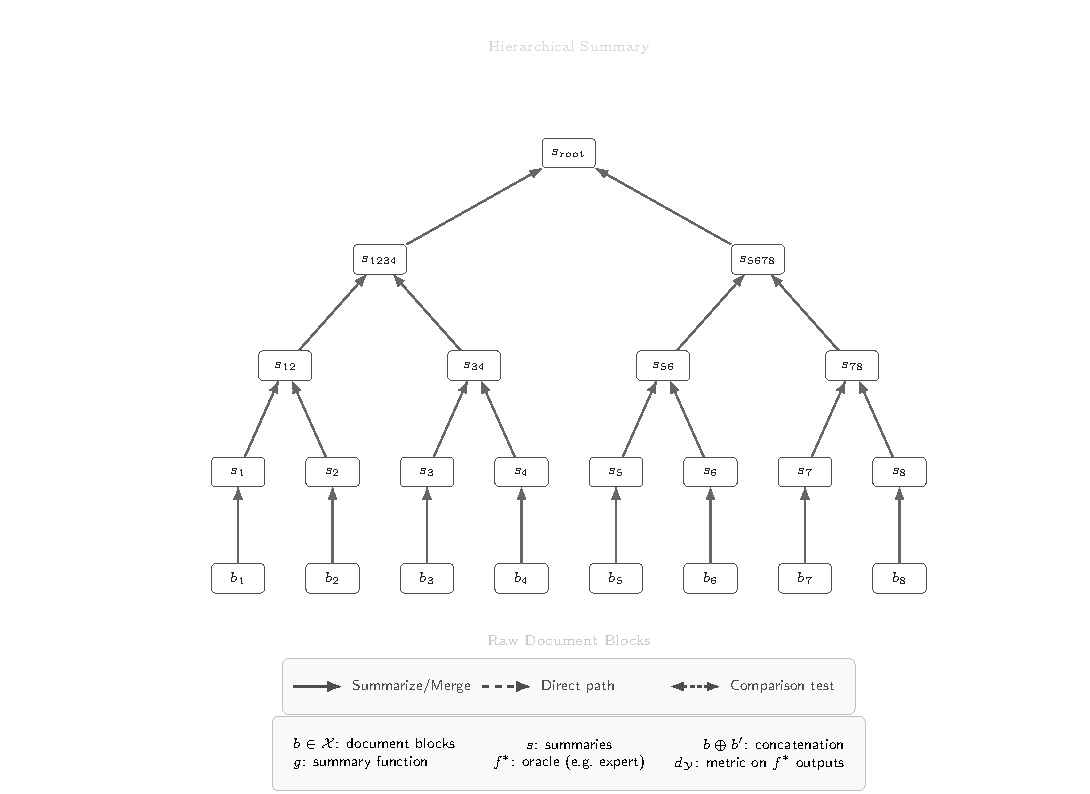
\includegraphics[width=\textwidth]{01_base.pdf}
    \caption{Base: Hierarchical Summarization Tree}
\end{figure}

\begin{figure}[h!]
    \centering
    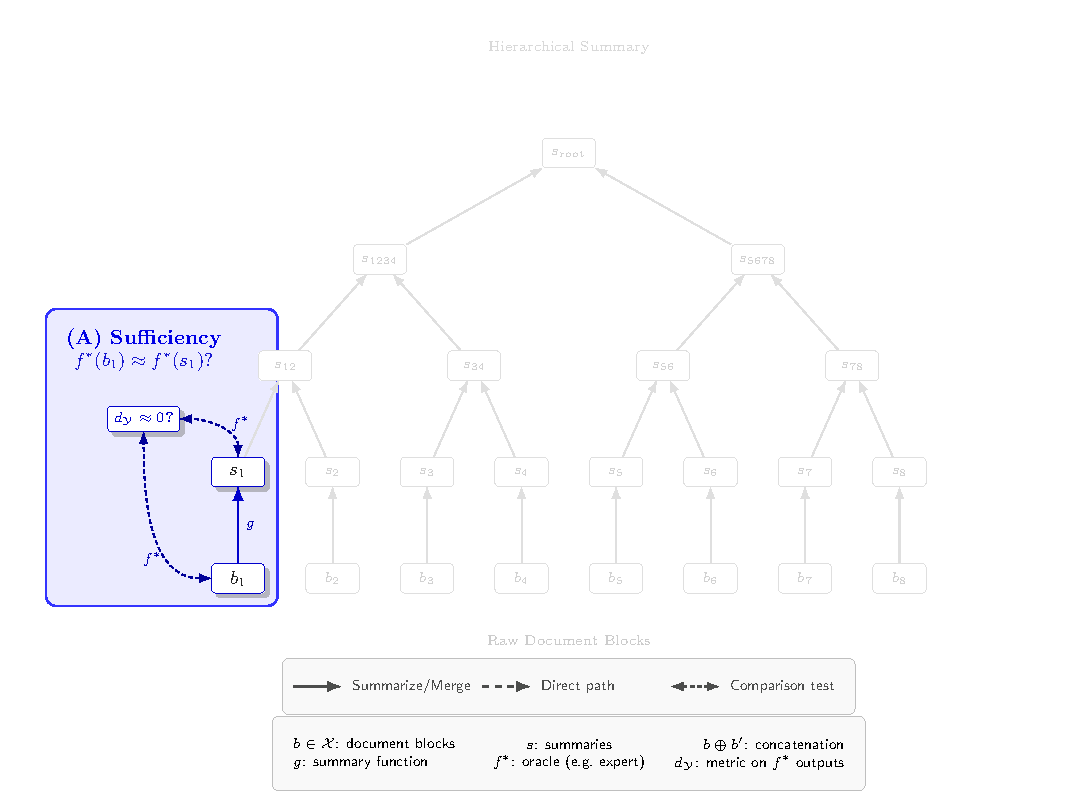
\includegraphics[width=\textwidth]{02_sufficiency.pdf}
    \caption{(A) Sufficiency: Does the summary preserve task-relevant information?}
\end{figure}

\begin{figure}[h!]
    \centering
    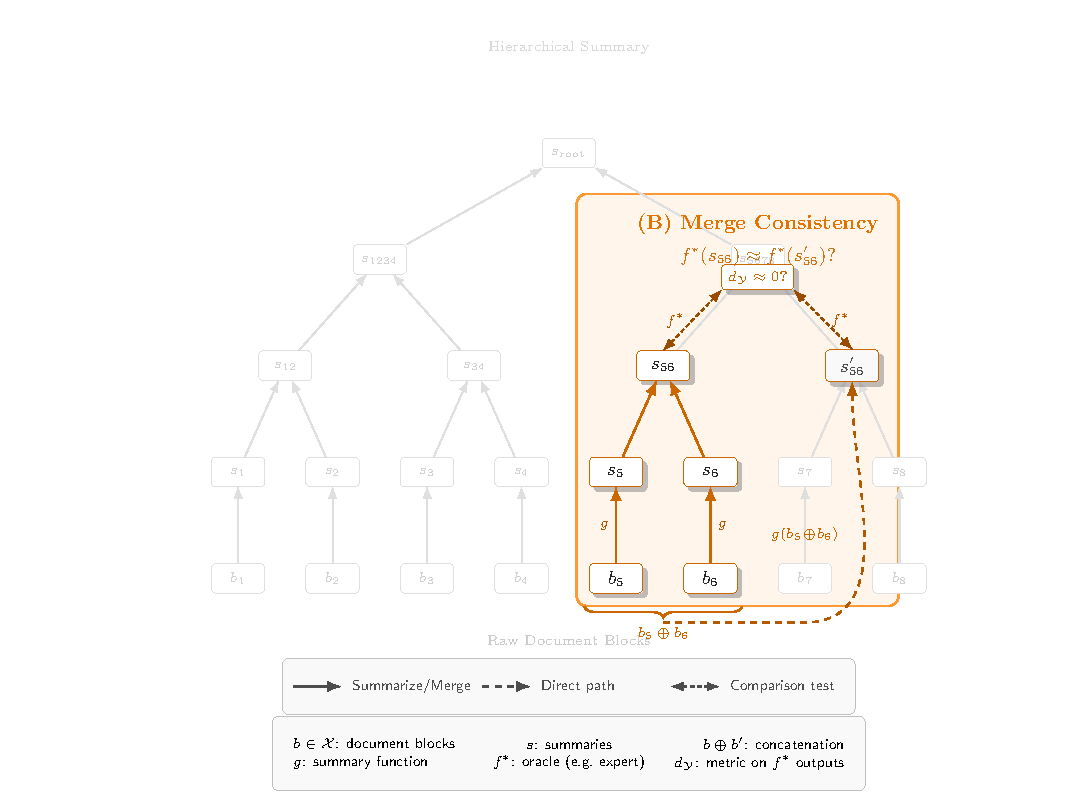
\includegraphics[width=\textwidth]{03_merge.pdf}
    \caption{(B) Merge Consistency: Is the merged summary equivalent to direct summarization?}
\end{figure}

\begin{figure}[h!]
    \centering
    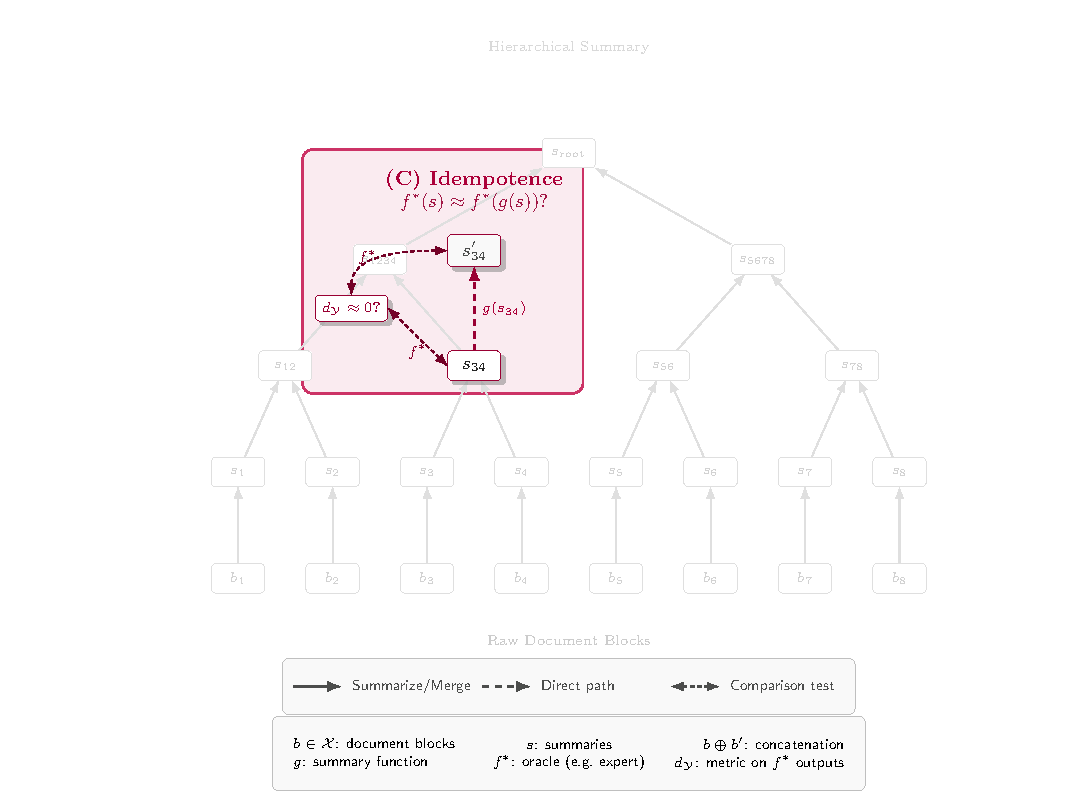
\includegraphics[width=\textwidth]{04_idempotence.pdf}
    \caption{(C) Idempotence: Is re-summarizing a summary stable?}
\end{figure}

\begin{figure}[h!]
    \centering
    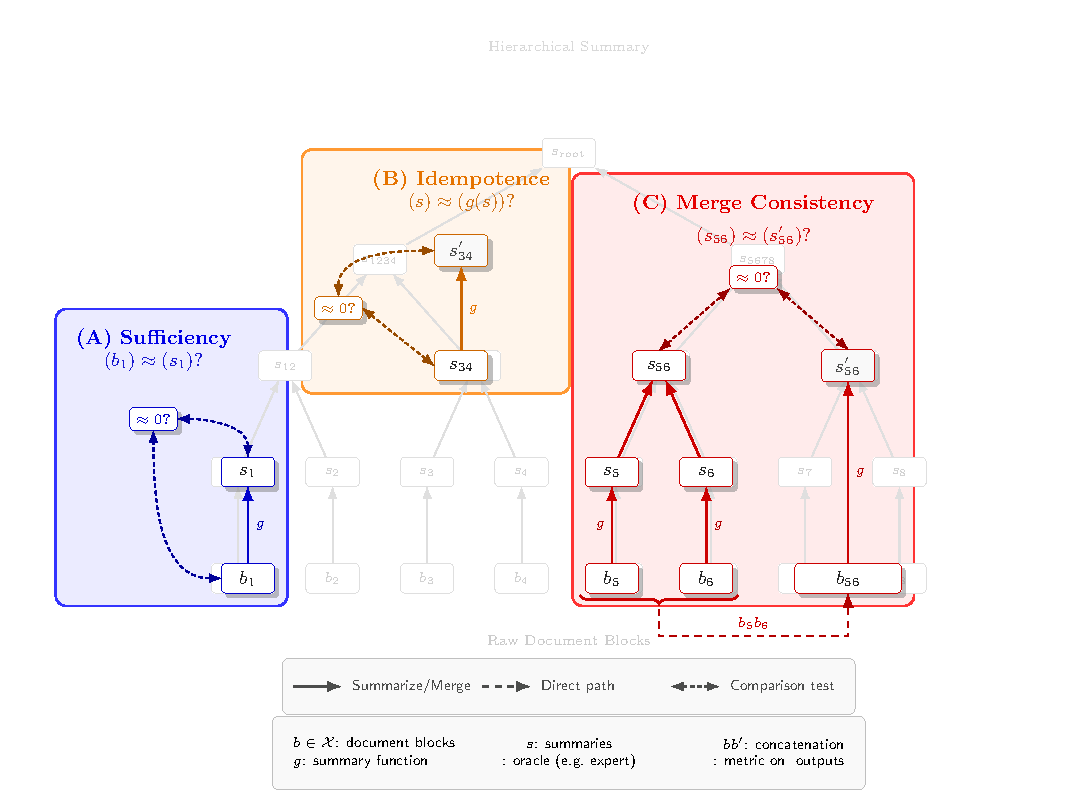
\includegraphics[width=\textwidth]{05_full.pdf}
    \caption{Full Figure: (A) Sufficiency + (B) Merge Consistency + (C) Idempotence}
\end{figure}

\end{document}
